% Provenance (never printed): cycle 4 (geographie and SVT, "La planete Terre"):
% why a flat map distorts, projections, scale, topographic maps and
% profiles, satellite images and satellite positioning; see
% sources/book1/PROVENANCE.md. Book 1, grade 9, chapter 5.
% Vocabulary guard: owns map projection (Mercator, equal-area), numerical
% scale and scale bar, topographic map, contour line and contour interval,
% remote sensing and satellite image, satellite positioning. "Scale" itself
% is g2's (drawing-to-map, Sync 1 ruling); globe and world map are g3's;
% parallels, meridians, latitude and longitude are g6's; altitude, relief
% and physical map are g4's; slope as a percentage was used in g9.2. The
% speed of light is the physics books' (recalled in prose). The V-rule of
% geological maps belongs to Book 3.
\chapter{Mapas da Terra inteira}\label{ch:g9:maps-of-the-earth}

Em muitos \omterm{def:g2:drawing-to-map:map}{mapas} de parede das salas de aula, a Groenlândia parece mais ou
menos tão grande quanto a África. Num \omterm{def:g3:continents-and-oceans:globe}{globo}, a África é cerca de catorze
vezes maior: cerca de 29~milhões de quilômetros quadrados para a África
continental, contra cerca de 2.1~milhões para a Groenlândia. Os dois são
imagens fiéis da Terra, feitas com cuidado. Então, qual deles está
mentindo, e por quê?
% ledger: data:ne-land (areas computed in figdata/grade-9/projections.py)

\begin{recall}
Um \omterm{def:g2:drawing-to-map:map}{mapa} é um desenho de um lugar visto de cima, menor que o lugar, com uma
\omterm{def:g2:drawing-to-map:legend}{legenda} e uma \omterm{def:g2:drawing-to-map:scale}{escala} (\cref{ch:g2:drawing-to-map}). Um \omterm{def:g3:continents-and-oceans:globe}{globo} é um pequeno
modelo da Terra redonda; um \omterm{def:g3:continents-and-oceans:world-map}{mapa-múndi} mostra a Terra inteira plana, numa
só imagem (\cref{ch:g3:continents-and-oceans}). Os \omterm{def:g6:latitude-longitude:latitude}{paralelos} e os
\omterm{def:g6:latitude-longitude:longitude}{meridianos} dão a cada lugar a sua \omterm{def:g6:latitude-longitude:latitude}{latitude} e a sua \omterm{def:g6:latitude-longitude:longitude}{longitude}
(\cref{ch:g6:latitude-longitude}). A \omterm{def:g4:world-physical-map:altitude}{altitude} é a altura acima do \omterm{def:g4:world-physical-map:altitude}{nível do
mar}, e um \omterm{def:g4:world-physical-map:physical-map}{mapa físico} mostra o \omterm{def:g4:world-physical-map:relief}{relevo} em cores
(\cref{ch:g4:world-physical-map}). Em física, você aprende que a luz
viaja a cerca de \qty{300000}{km} por segundo.
\end{recall}
% ledger: const:c

\section{Por que um mapa plano tem de deformar}

Tente achatar a casca de uma laranja sobre uma mesa: ela rasga ou estica.
A superfície de uma esfera não pode ser estendida no plano sem mudar
alguns comprimentos. Para desenhar a Terra inteira numa folha, o
cartógrafo escolhe uma regra que leva cada ponto do \omterm{def:g3:continents-and-oceans:globe}{globo} a um ponto da
folha, e escolhe o que o \omterm{def:g2:drawing-to-map:map}{mapa} vai manter fiel e o que ele vai sacrificar.

\begin{definition}[Projeção cartográfica]\label{def:g9:maps-of-the-earth:projection}
Uma \emph{projeção cartográfica}\index{projecao cartografica@projeção cartográfica}
é uma regra que leva cada ponto do \omterm{def:g3:continents-and-oceans:globe}{globo}, dado pela sua \omterm{def:g6:latitude-longitude:latitude}{latitude} e pela
sua \omterm{def:g6:latitude-longitude:longitude}{longitude}, a um ponto de um \omterm{def:g2:drawing-to-map:map}{mapa} plano. Numa \emph{projeção de
Mercator}\index{projecao de Mercator@projeção de Mercator}, os \omterm{def:g6:latitude-longitude:latitude}{paralelos} e
os \omterm{def:g6:latitude-longitude:longitude}{meridianos} são retas que se cruzam em ângulo reto, e a forma de cada
pequena região é mantida, mas as áreas são ampliadas cada vez mais em
direção aos \omterm{def:g3:continents-and-oceans:poles}{polos}. Numa \emph{projeção
equivalente}\index{projecao equivalente@projeção equivalente}, cada
região mantém a sua área verdadeira em relação às outras, mas as formas
são entortadas, cada vez mais em direção às bordas do \omterm{def:g2:drawing-to-map:map}{mapa}.
\end{definition}

A figura abaixo desenha nos dois \omterm{def:g2:drawing-to-map:map}{mapas} os mesmos círculos iguais do \omterm{def:g3:continents-and-oceans:globe}{globo},
todos do mesmo tamanho. No \omterm{def:g2:drawing-to-map:map}{mapa} de Mercator, os círculos continuam
redondos, mas crescem em direção aos \omterm{def:g3:continents-and-oceans:poles}{polos}: na \omterm{def:g6:latitude-longitude:latitude}{latitude} \ang{60}, a sua
área é quatro vezes a área no \omterm{def:g3:continents-and-oceans:equator}{equador}, e perto do meio da Groenlândia, a
cerca de \ang{72}, cerca de dez vezes. No \omterm{def:g2:drawing-to-map:map}{mapa} equivalente, os círculos
mantêm todos a mesma área, mas os que ficam longe do centro são achatados
em ovais.
% ledger: data:ne-land (circles and factors computed in figdata/grade-9/projections.py, mercator_area_factor)

Nenhuma projeção é a melhor para tudo. A \omterm{def:g9:maps-of-the-earth:projection}{projeção de Mercator} foi feita
para os navegadores: um rumo que mantém a mesma direção da bússola é uma
reta nela. Para comparar os tamanhos de países, de florestas ou de
\omterm{def:g5:weather-and-climate:desert}{desertos}, um \omterm{def:g2:drawing-to-map:map}{mapa} equivalente diz a verdade. Antes de confiar num
\omterm{def:g3:continents-and-oceans:world-map}{mapa-múndi}, vale a pena perguntar que projeção ele usa.

\begin{omfigure}
\begin{tikzpicture}
\begin{axis}[name=merc, x=0.0215cm, y=0.0215cm, xmin=-180, xmax=180,
  ymin=-140, ymax=169, axis line style={black!50}, ticks=none,
  title={\footnotesize projeção de Mercator}, title style={yshift=-1ex}]
  \addplot[black!15, line width=0.3pt] table {figdata/out/grade-9-projections-merc-grid.dat};
  \addplot[fill=black!25, draw=black!45, line width=0.15pt] table {figdata/out/grade-9-projections-merc-land.dat};
  \addplot[fill=orange!55, draw=orange!70!black, line width=0.3pt] table {figdata/out/grade-9-projections-merc-greenland.dat};
  \addplot[fill=blue!30, draw=blue!60!black, line width=0.3pt] table {figdata/out/grade-9-projections-merc-africa.dat};
  \addplot[red!80!black, line width=0.6pt] table {figdata/out/grade-9-projections-merc-circles.dat};
\end{axis}
\begin{axis}[at={(merc.east)}, anchor=west, xshift=0.3cm, x=0.025cm, y=0.025cm,
  xmin=-165, xmax=165, ymin=-83, ymax=83, hide axis,
  title={\footnotesize uma projeção equivalente}, title style={yshift=-1ex}]
  \addplot[black!15, line width=0.3pt] table {figdata/out/grade-9-projections-moll-grid.dat};
  \addplot[fill=black!25, draw=black!45, line width=0.15pt] table {figdata/out/grade-9-projections-moll-land.dat};
  \addplot[fill=orange!55, draw=orange!70!black, line width=0.3pt] table {figdata/out/grade-9-projections-moll-greenland.dat};
  \addplot[fill=blue!30, draw=blue!60!black, line width=0.3pt] table {figdata/out/grade-9-projections-moll-africa.dat};
  \addplot[red!80!black, line width=0.6pt] table {figdata/out/grade-9-projections-moll-circles.dat};
\end{axis}
\end{tikzpicture}

{\small O mesmo mundo em duas projeções. Em vermelho: círculos do mesmo
tamanho no \omterm{def:g3:continents-and-oceans:globe}{globo}, centrados a cada \ang{30} de \omterm{def:g6:latitude-longitude:latitude}{latitude} e a cada \ang{60}
de \omterm{def:g6:latitude-longitude:longitude}{longitude}. Em laranja: a Groenlândia; em azul: a África continental.
No \omterm{def:g2:drawing-to-map:map}{mapa} de Mercator (à esquerda, cortado em \ang{80}\,S e \ang{84}\,N,
porque os \omterm{def:g3:continents-and-oceans:poles}{polos} ficariam infinitamente longe), os dois parecem mais ou
menos do mesmo tamanho; no \omterm{def:g2:drawing-to-map:map}{mapa} equivalente (à direita), a África é cerca
de 14 vezes maior, como no \omterm{def:g3:continents-and-oceans:globe}{globo}. Litorais do Natural Earth.}
% ledger: data:ne-land
\label{fig:g9:maps-of-the-earth:projections}
\end{omfigure}

\begin{example}[A Groenlândia e a África]
A África continental cobre cerca de 29~milhões de~\unit{km^2}, a
Groenlândia cerca de 2.1~milhões de~\unit{km^2}: $29 \div 2.1 \approx 14$.
A África fica dos dois lados do \omterm{def:g3:continents-and-oceans:equator}{equador}, onde a \omterm{def:g9:maps-of-the-earth:projection}{projeção de Mercator} quase
não amplia nada, enquanto a maior parte da Groenlândia fica entre cerca de
\ang{60} e \ang{84} norte, onde as áreas são ampliadas de 4 a mais de 10
vezes. No \omterm{def:g2:drawing-to-map:map}{mapa} de Mercator, as duas saem mais ou menos do mesmo tamanho.
\end{example}
% ledger: data:ne-land (areas and ratios computed in figdata/grade-9/projections.py, areas)

\section{A escala}

O \omterm{def:g2:drawing-to-map:map}{mapa} de um \omterm{def:g1:landscapes-around-us:landform}{vale} ou de uma cidade é um pedaço tão pequeno da Terra que a
projeção quase não importa. O que importa é quantas vezes o \omterm{def:g2:drawing-to-map:map}{mapa} é menor
que o terreno.

\begin{definition}[Escala numérica e escala gráfica]\label{def:g9:maps-of-the-earth:numerical-scale}
A \emph{escala numérica}\index{escala numerica@escala numérica} de um
\omterm{def:g2:drawing-to-map:map}{mapa} é uma razão como $1 : 25\,000$: um centímetro no \omterm{def:g2:drawing-to-map:map}{mapa} representa
\num{25000} centímetros no terreno, e o mesmo vale para qualquer unidade.
Uma \emph{escala gráfica}\index{escala grafica@escala gráfica} é uma
régua desenhada no \omterm{def:g2:drawing-to-map:map}{mapa}, marcada com as distâncias no terreno.
\end{definition}

\begin{method}[Usar uma escala numérica]
\begin{enumerate}
  \item Meça a distância no \omterm{def:g2:drawing-to-map:map}{mapa}, em centímetros.
  \item Multiplique-a pelo número depois dos dois-pontos: o resultado é a
        distância no terreno, em centímetros.
  \item Converta: divida por 100 para ter metros, por \num{100000} para
        ter quilômetros.
\end{enumerate}
\end{method}

\begin{example}[Um passeio num mapa a $1 : 25\,000$]
Num \omterm{def:g2:drawing-to-map:map}{mapa} a $1 : 25\,000$, uma trilha mede \qty{6}{cm}. No terreno, ela
tem $6 \times 25\,000 = \num{150000}$~cm, ou seja, \qty{1500}{m} ou
\qty{1.5}{km}. Cada centímetro do \omterm{def:g2:drawing-to-map:map}{mapa} representa \qty{250}{m}.
\end{example}

A \omterm{def:g9:maps-of-the-earth:numerical-scale}{escala gráfica} tem uma vantagem sobre a \omterm{def:g9:maps-of-the-earth:numerical-scale}{escala numérica}: quando um \omterm{def:g2:drawing-to-map:map}{mapa}
é ampliado ou reduzido numa tela ou numa copiadora, a régua é ampliada ou
reduzida junto com ele e continua certa, enquanto a razão impressa no
canto fica errada.

\section{O mapa topográfico}

Um \omterm{def:g4:world-physical-map:physical-map}{mapa físico} mostra o \omterm{def:g4:world-physical-map:relief}{relevo} com cores. Um \omterm{def:g2:drawing-to-map:map}{mapa} de uma área pequena o
mostra com muito mais precisão, com linhas.

\begin{definition}[Mapa topográfico]\label{def:g9:maps-of-the-earth:topographic-map}
Um \emph{mapa topográfico}\index{mapa topografico@mapa topográfico} é um
\omterm{def:g2:drawing-to-map:map}{mapa} detalhado de uma área pequena, numa \omterm{def:g2:drawing-to-map:scale}{escala} como $1 : 25\,000$ ou
$1 : 50\,000$, que mostra a forma e a altura do terreno, com os \omterm{def:g1:landscapes-around-us:water}{rios}, as
estradas, as trilhas, as construções e os bosques.
\end{definition}

\begin{definition}[Curva de nível e equidistância]\label{def:g9:maps-of-the-earth:contour}
Uma \emph{curva de nível}\index{curva de nivel@curva de nível} é uma
linha num \omterm{def:g2:drawing-to-map:map}{mapa} que liga pontos do terreno de mesma \omterm{def:g4:world-physical-map:altitude}{altitude}. A
\emph{equidistância}\index{equidistancia@equidistância} é a diferença de
\omterm{def:g4:world-physical-map:altitude}{altitude} entre duas curvas de nível vizinhas; ela é a mesma no \omterm{def:g2:drawing-to-map:map}{mapa}
inteiro.
\end{definition}

Imagine um morro fatiado por planos horizontais, um a cada \qty{100}{m}.
Cada fatia corta o morro ao longo de uma linha fechada; vistas de cima,
essas linhas são as \omterm{def:g9:maps-of-the-earth:contour}{curvas de nível}.

\begin{omfigure}
\begin{tikzpicture}[font=\footnotesize]
  % side view
  \fill[black!13] (0,0) .. controls (1.2,0.3) and (2.0,1.3) .. (2.8,2.2)
     .. controls (3.2,2.6) and (3.5,2.6) .. (3.7,2.2) .. controls (3.9,1.6) and (4.1,0.4) .. (4.5,0) -- cycle;
  \draw[black!70] (0,0) .. controls (1.2,0.3) and (2.0,1.3) .. (2.8,2.2)
     .. controls (3.2,2.6) and (3.5,2.6) .. (3.7,2.2) .. controls (3.9,1.6) and (4.1,0.4) .. (4.5,0);
  \draw[black!70] (-0.3,0) -- (4.9,0);
  \foreach \y/\h in {0.6/100, 1.2/200, 1.8/300} {
    \draw[omContour, dashed] (-0.3,\y) -- (4.9,\y);
    \node[anchor=east, omContour] at (-0.3,\y) {\h~m};
  }
  \node[anchor=south] at (3.3,2.5) {vista de lado};
  \node[anchor=north] at (1.4,-0.05) {suave a oeste};
  \node[anchor=north] at (4.1,-0.05) {íngreme a leste};
  % map view
  \begin{scope}[xshift=8.4cm, yshift=1.3cm]
    \draw[omContour, line width=0.5pt] (0.25,0) ellipse (2.1 and 1.25);
    \draw[omContour, line width=0.5pt] (0.75,0.02) ellipse (1.3 and 0.9);
    \draw[omContour, line width=0.5pt] (1.05,0.04) ellipse (0.62 and 0.5);
    \fill (1.25,0.05) circle (0.04);
    \draw[black!60] (1.25,0.05) -- (2.9,-0.6) node[anchor=west, inner sep=1.5pt] {cume};
    \node[omContour, fill=white, inner sep=0.5pt] at (-1.85,0) {100};
    \node[omContour, fill=white, inner sep=0.5pt] at (-0.55,0) {200};
    \node[omContour, fill=white, inner sep=0.5pt] at (0.43,0) {300};
    \node[anchor=north] at (0.25,-1.35) {vista de cima: as curvas de nível};
    \draw[->] (2.7,0.9) -- (2.7,1.4) node[above] {N};
  \end{scope}
\end{tikzpicture}

{\small Um morro fatiado a cada \qty{100}{m} (um esboço). Visto de cima,
cada fatia dá uma \omterm{def:g9:maps-of-the-earth:contour}{curva de nível} fechada em volta do cume. Onde a encosta
é íngreme (leste), as curvas ficam juntas; onde ela é suave (oeste), elas
ficam afastadas.}
\label{fig:g9:maps-of-the-earth:slices}
\end{omfigure}

Um \omterm{def:g9:maps-of-the-earth:topographic-map}{mapa topográfico} se lê com algumas regras.
\begin{itemize}
  \item As \omterm{def:g9:maps-of-the-earth:contour}{curvas de nível} nunca se cruzam: um ponto só tem uma \omterm{def:g4:world-physical-map:altitude}{altitude}.
  \item Quanto mais juntas as \omterm{def:g9:maps-of-the-earth:contour}{curvas de nível}, mais íngreme a encosta;
        afastadas, o terreno é suave; sem nenhuma curva, ele é quase plano.
  \item Linhas fechadas umas dentro das outras, subindo para o centro,
        marcam um morro; o seu topo muitas vezes é marcado por um ponto com
        a sua \omterm{def:g4:world-physical-map:altitude}{altitude}, um \emph{ponto cotado}.
  \item Onde uma \omterm{def:g9:maps-of-the-earth:contour}{curva de nível} atravessa um \omterm{def:g1:landscapes-around-us:landform}{vale}, ela se dobra \omterm{def:g1:landscapes-around-us:water}{rio} acima,
        num V que aponta para a cabeceira do \omterm{def:g1:landscapes-around-us:landform}{vale}.
  \item A cada cinco curvas, a \emph{curva mestra} é desenhada mais grossa
        e marcada com a sua \omterm{def:g4:world-physical-map:altitude}{altitude}.
\end{itemize}

A declividade do terreno entre dois pontos é a subida dividida pela
distância horizontal, muitas vezes escrita como porcentagem. No \omterm{def:g2:drawing-to-map:map}{mapa}
abaixo, indo para o norte a partir do \omterm{def:g1:landscapes-around-us:water}{rio}, as curvas de \qty{200}{m} e de
\qty{400}{m} na linha C--D ficam a cerca de \qty{0.75}{km} uma da outra:
a declividade é de cerca de $200 \div 750
\approx 0.27$, ou \qty{27}{\%}.
% ledger: (invented region: crossings 2.09 and 2.83 km from C, figdata/grade-9/varden_topo.py)

\begin{method}[Desenhar um perfil topográfico]
\begin{enumerate}
  \item Trace a linha do perfil no \omterm{def:g2:drawing-to-map:map}{mapa}, de uma ponta (C) à outra (D).
  \item Encoste a borda reta de uma tira de papel ao longo da linha; marque
        C, D e cada ponto onde a linha cruza uma \omterm{def:g9:maps-of-the-earth:contour}{curva de nível}, com a sua
        \omterm{def:g4:world-physical-map:altitude}{altitude}.
  \item Desenhe um eixo horizontal do comprimento de C--D (as distâncias)
        e um eixo vertical de \omterm{def:g4:world-physical-map:altitude}{altitudes}.
  \item Leve cada marca para o gráfico, à sua distância de C e na sua
        \omterm{def:g4:world-physical-map:altitude}{altitude}, e ligue os pontos com uma curva suave: arredondada nos
        topos dos morros, plana ao longo do fundo de um \omterm{def:g1:landscapes-around-us:landform}{vale}.
\end{enumerate}
\end{method}

\begin{omfigure}
\begin{tikzpicture}
\begin{axis}[name=map, x=2cm, y=2cm, xmin=2, xmax=8, ymin=1.8, ymax=6.2, ticks=none,
  axis line style={black!60}, clip mode=individual]
  \addplot[contour] table {figdata/out/shared-region-contours.dat};
  \addplot[index contour] table {figdata/out/shared-region-index-contours.dat};
  \addplot[river] table {figdata/out/shared-region-river.dat};
  \addplot[only marks, mark=none, point meta=explicit symbolic, nodes near coords,
    nodes near coords align={center}, nodes near coords style={font=\tiny, fill=white, inner sep=0.6pt, text=omContour}]
    table[meta=label] {figdata/out/grade-9-varden_topo-labels.dat};
  \addplot[only marks, mark=*, mark size=1.2pt, point meta=explicit symbolic, nodes near coords,
    nodes near coords align={right}, nodes near coords style={font=\scriptsize, inner sep=1.5pt}]
    table[meta=label] {figdata/out/grade-9-varden_topo-spots.dat};
  \addplot[black, line width=0.8pt] table[x=x_km, y=y_km] {figdata/out/grade-9-varden_topo-cd.dat};
  \addplot[only marks, mark=none, point meta=explicit symbolic, nodes near coords,
    nodes near coords align={left}, nodes near coords style={font=\small\bfseries, inner sep=2pt}]
    table[meta=label] {figdata/out/grade-9-varden_topo-cd.dat};
  \coordinate (na) at (axis cs:8.3,5.3);
  \coordinate (sb) at (axis cs:2.2,1.95);
\end{axis}
\pic at (na) {northarrow};
\fill[white] ($(sb)+(-0.1,-0.42)$) rectangle ($(sb)+(2.3,0.25)$);
\pic at (sb) {scalebar={2}{1 km}};
\node[anchor=west, font=\footnotesize, fill=white, inner sep=1pt] at ($(sb)+(2.35,0.06)$) {$1 : 50\,000$};
\begin{axis}[at={(map.south)}, anchor=north, yshift=-0.9cm, x=2cm, y=0.006cm, clip=false,
  xmin=0, xmax=4, ymin=100, ymax=600, axis x line=bottom, axis y line=left,
  axis line style={-}, grid=major, grid style={black!12},
  xtick={0,1,2,3,4}, ytick={100,200,...,600}, tick label style={font=\scriptsize},
  xlabel={distância a partir de C (km)}, ylabel={altitude (m)}, label style={font=\footnotesize}]
  \addplot[black!70, line width=0.8pt] table[x=s_km, y=z_m] {figdata/out/grade-9-varden_topo-profile.dat};
  \addplot[only marks, mark=*, mark size=1.1pt, omContour] table[x=s_km, y=z_m] {figdata/out/grade-9-varden_topo-cross.dat};
  \node[font=\small\bfseries, anchor=south] at (axis cs:0,600) {C};
  \node[font=\small\bfseries, anchor=south] at (axis cs:4,600) {D};
\end{axis}
\end{tikzpicture}

{\small Em cima: um \omterm{def:g9:maps-of-the-earth:topographic-map}{mapa topográfico} de uma parte das Colinas de Varden a
$1 : 50\,000$ (1~cm no \omterm{def:g2:drawing-to-map:map}{mapa} para \qty{500}{m} no terreno). \omterm{def:g9:maps-of-the-earth:contour}{Equidistância}
de \qty{50}{m}; as curvas mestras, mais grossas, estão em 250 e
\qty{500}{m}. O \omterm{def:g1:landscapes-around-us:water}{rio} corre para leste ao longo de um fundo de \omterm{def:g1:landscapes-around-us:landform}{vale} plano.
Embaixo: o perfil topográfico ao longo de C--D, de sul para norte; os
pontos são os lugares onde C--D cruza uma \omterm{def:g9:maps-of-the-earth:contour}{curva de nível} (a escala
vertical está esticada três vezes).}
% ledger: (invented region: the Varden Hills, figdata/shared/region.py; labels, spot height and profile from figdata/grade-9/varden_topo.py)
\label{fig:g9:maps-of-the-earth:topo}
\end{omfigure}

\section{As imagens de satélite da Terra}

Em 23~de~julho de 1972, um foguete lançou o primeiro satélite construído
para estudar a superfície da Terra, mais tarde chamado Landsat~1. Dando
14 voltas na Terra por dia a \qty{917}{km} de \omterm{def:g4:world-physical-map:altitude}{altitude}, de \omterm{def:g3:continents-and-oceans:poles}{polo} a \omterm{def:g3:continents-and-oceans:poles}{polo},
ele passava sobre o mesmo lugar a cada 18 dias e, em seis anos, tirou
imagens de cerca de três quartos da superfície da Terra. Os satélites
Landsat fotografam as terras sem interrupção desde então.
% ledger: usgs:landsat1

\begin{definition}[Sensoriamento remoto e imagem de satélite]\label{def:g9:maps-of-the-earth:remote-sensing}
O \emph{sensoriamento remoto}\index{sensoriamento remoto} é a observação
da Terra à distância, de aviões ou de satélites, medindo a luz e as
outras radiações que a superfície devolve. Uma \emph{imagem de
satélite}\index{imagem de satelite@imagem de satélite} é uma imagem de
uma parte da Terra construída a partir dessas medidas.
\end{definition}

A câmera de um satélite vê mais que os nossos olhos: ela também mede a luz
infravermelha, que é invisível. Mostrado em cores na imagem (uma imagem em
\emph{falsa cor}), o infravermelho revela as plantas, o solo úmido ou a
\omterm{def:g3:stones-pebbles-sand:rock}{rocha} nua. Imagens do mesmo lugar tiradas com anos de intervalo mostram
como um \omterm{def:g1:landscapes-around-us:water}{litoral}, uma floresta, uma \omterm{def:g8:ice-on-earth:glacier}{geleira} ou uma cidade muda
(\cref{ch:g8:ice-on-earth}).

\begin{omfigure}
\begin{minipage}[c]{0.5\linewidth}\centering
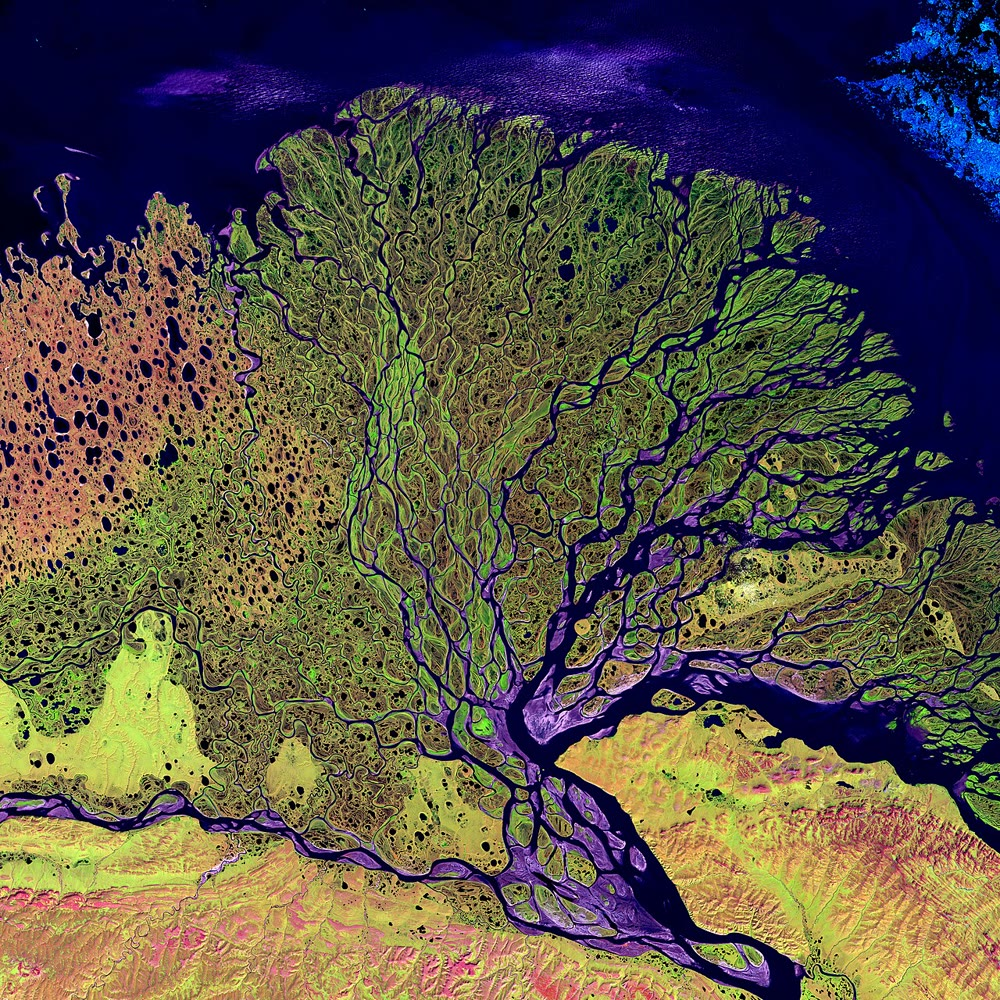
\includegraphics[width=\linewidth]{images/book1/g9-lena-delta.jpg}
\end{minipage}\hfill
\begin{minipage}[c]{0.46\linewidth}\raggedright
{\small O \omterm{def:g5:water-shapes-the-land:delta}{delta} do \omterm{def:g1:landscapes-around-us:water}{rio} Lena, na Sibéria, onde ele encontra o \omterm{def:g2:water-on-earth:ocean}{oceano}
Ártico: uma imagem Landsat em falsa cor de 27~de~fevereiro de 2000, feita
com infravermelho de ondas curtas, infravermelho e luz vermelha. Os muitos
canais do \omterm{def:g1:landscapes-around-us:water}{rio} aparecem em azul. USGS EROS Data Center, via NASA Visible
Earth (domínio público, via Wikimedia Commons).}
\end{minipage}
% ledger: commons:lena-landsat
\label{fig:g9:maps-of-the-earth:lena}
\end{omfigure}

\section{O posicionamento por satélite}

Um celular ou um carro consegue dizer onde está com uma precisão de alguns
metros, em quase qualquer lugar da Terra. Ele não vê os satélites; ele os
escuta.

\begin{definition}[Posicionamento por satélite]\label{def:g9:maps-of-the-earth:positioning}
O \emph{posicionamento por satélite}\index{posicionamento por satelite@posicionamento por satélite}
é encontrar uma posição na Terra a partir das distâncias a vários
satélites cujas posições são conhecidas. Um receptor calcula cada
distância a partir do tempo que um sinal do satélite leva para chegar até
ele.
\end{definition}

O sistema americano, o GPS, mantém pelo menos 24 satélites em
funcionamento a uma \omterm{def:g4:world-physical-map:altitude}{altitude} de cerca de \qty{20200}{km}. Cada um dá duas
voltas na Terra por dia, em seis órbitas distribuídas em volta do
planeta, de modo que, de quase qualquer ponto da Terra, pelo menos quatro
satélites estão à vista. Um sinal vindo de \qty{20200}{km}, viajando à
velocidade da luz, chega depois de $20\,200 \div
300\,000 \approx 0.067$~s: o receptor mede esse tempo e o transforma em
distância.
% ledger: gps:constellation, const:c (travel time computed in figdata/grade-9/trilateration.py)

Como as distâncias dão uma posição? Imagine a ideia num \omterm{def:g2:drawing-to-map:map}{mapa} plano. Se o
receptor está a \qty{5}{km} da baliza~A, ele fica em algum lugar de um
círculo de raio \qty{5}{km} em volta de A. Se ele também está a
\qty{10}{km} de B, ele fica nos dois círculos: num dos dois pontos onde
eles se cruzam. Uma terceira distância, \qty{5}{km} de C, escolhe o
ponto certo. No espaço, os círculos viram esferas, e é preciso mais um
satélite pela mesma razão.

\begin{omfigure}
\begin{minipage}[c]{0.5\linewidth}\centering
\begin{tikzpicture}
\begin{axis}[x=0.42cm, y=0.42cm, xmin=-1, xmax=13, ymin=-1.5, ymax=13,
  ticks=none, axis line style={black!40}]
  \addplot[omSea!70!black, line width=0.6pt] table {figdata/out/grade-9-trilateration-circles.dat};
  \addplot[only marks, mark=triangle*, mark size=2.6pt, point meta=explicit symbolic, nodes near coords,
    nodes near coords style={font=\footnotesize\bfseries, anchor=south west, inner sep=1pt}]
    table[meta=label] {figdata/out/grade-9-trilateration-beacons.dat};
  % labels first (on a white patch), then the points on top of them
  \addplot[only marks, mark=none, point meta=explicit symbolic, nodes near coords,
    nodes near coords style={font=\footnotesize\bfseries, anchor=north east, xshift=-1pt, yshift=-1pt, inner sep=1pt, fill=white, text=red!75!black}, skip coords between index={1}{2}]
    table[meta=label] {figdata/out/grade-9-trilateration-points.dat};
  \addplot[only marks, mark=none, point meta=explicit symbolic, nodes near coords,
    nodes near coords style={font=\footnotesize, anchor=south west, xshift=1pt, yshift=1pt, inner sep=1pt, fill=white}, skip coords between index={0}{1}]
    table[meta=label] {figdata/out/grade-9-trilateration-points.dat};
  \addplot[only marks, mark=*, mark size=2pt, red!75!black, skip coords between index={1}{2}] table {figdata/out/grade-9-trilateration-points.dat};
  \addplot[only marks, mark=o, mark size=2pt, fill=white, skip coords between index={0}{1}] table {figdata/out/grade-9-trilateration-points.dat};
\end{axis}
\end{tikzpicture}
\end{minipage}\hfill
\begin{minipage}[c]{0.46\linewidth}\raggedright
{\small O posicionamento num \omterm{def:g2:drawing-to-map:map}{mapa} plano (um esboço; a quadrícula em
quilômetros não está desenhada). O receptor R está a \qty{5}{km} de A, a
\qty{10}{km} de B e a \qty{5}{km} de C. Os círculos em volta de A e de B
se cruzam em R e num ponto falso F; só R também fica no círculo em volta
de C.}
\end{minipage}
% ledger: (invented region: exercise data, figdata/grade-9/trilateration.py)
\label{fig:g9:maps-of-the-earth:trilateration}
\end{omfigure}

\begin{omfigure}
\begin{minipage}[t]{0.48\linewidth}\centering
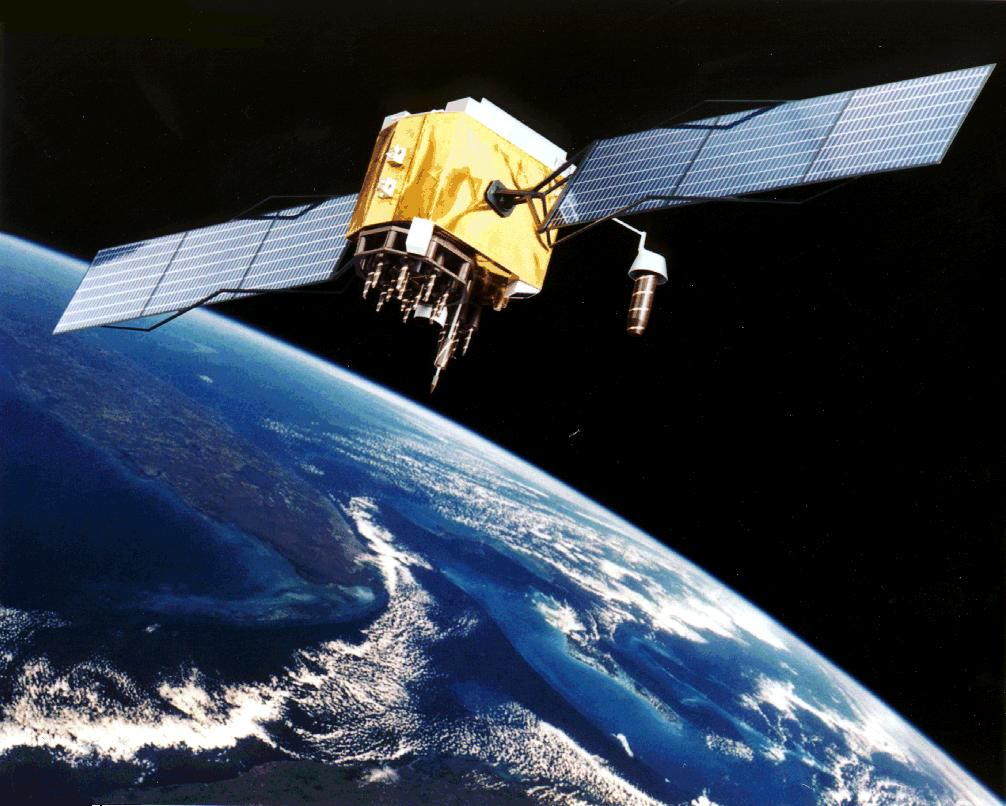
\includegraphics[width=\linewidth]{images/book1/g9-gps-satellite.jpg}

{\small Um satélite GPS em órbita, como um artista o imaginou. NASA
(domínio público, via Wikimedia Commons).}
\end{minipage}\hfill
\begin{minipage}[t]{0.48\linewidth}\centering
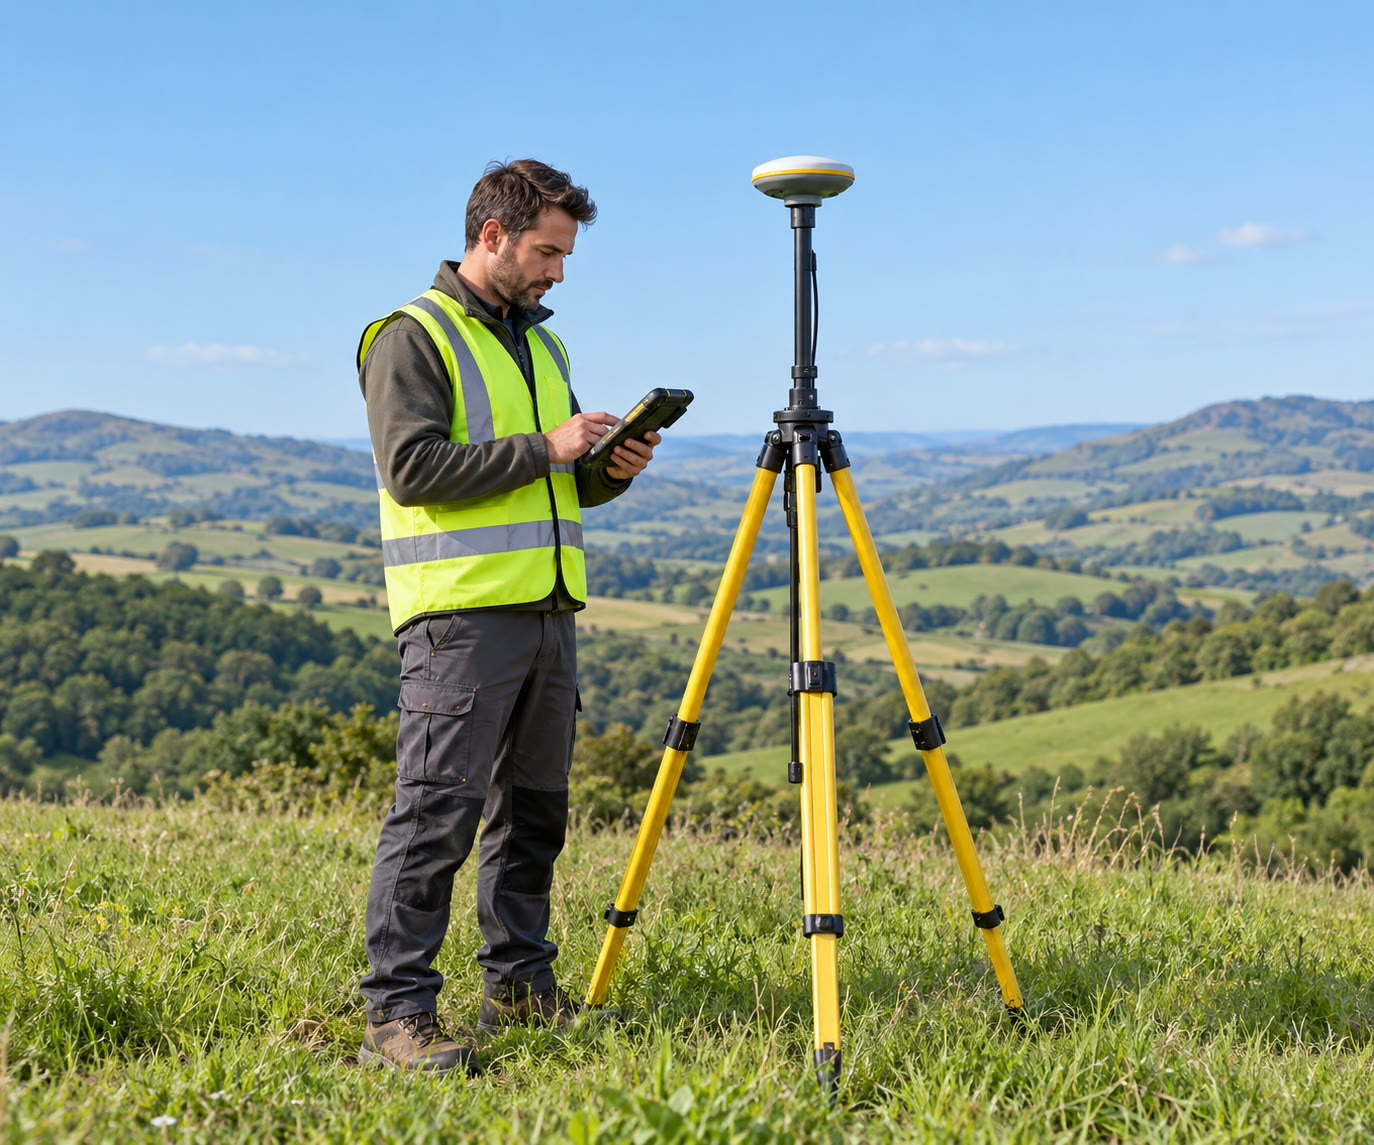
\includegraphics[width=\linewidth]{images/book1/ai/g9-surveyor.jpg}

{\small Um agrimensor fixa a posição de um ponto com um receptor de
satélite sobre um tripé (uma ilustração).}
\end{minipage}
% ledger: commons:gps-iif
\label{fig:g9:maps-of-the-earth:gps}
\end{omfigure}

\section{Exercícios}

\begin{exercise}[$\star$]\label{exo:g9:maps-of-the-earth:1}
Dê a palavra de cada descrição. (a) Uma regra que leva cada ponto do \omterm{def:g3:continents-and-oceans:globe}{globo}
a um ponto de um \omterm{def:g2:drawing-to-map:map}{mapa} plano. (b) Uma linha que liga pontos de mesma
\omterm{def:g4:world-physical-map:altitude}{altitude}. (c) Uma razão como $1 : 50\,000$. (d) A diferença de \omterm{def:g4:world-physical-map:altitude}{altitude}
entre duas \omterm{def:g9:maps-of-the-earth:contour}{curvas de nível} vizinhas. (e) Observar a Terra à distância,
por exemplo de um satélite.
\end{exercise}

\begin{exercise}[$\star$]\label{exo:g9:maps-of-the-earth:2}
Converta cada distância no \omterm{def:g2:drawing-to-map:map}{mapa} numa distância no terreno, em metros ou em
quilômetros. (a) \qty{4}{cm} num \omterm{def:g2:drawing-to-map:map}{mapa} a $1 : 25\,000$. (b) \qty{3}{cm}
num \omterm{def:g2:drawing-to-map:map}{mapa} a $1 : 50\,000$. (c) \qty{2.5}{cm} num \omterm{def:g2:drawing-to-map:map}{mapa} a $1 : 1\,000\,000$.
(d) Num \omterm{def:g2:drawing-to-map:map}{mapa} a $1 : 25\,000$, quantos centímetros representam
\qty{1}{km}?
\end{exercise}

\begin{exercise}[$\star$]\label{exo:g9:maps-of-the-earth:3}
Verdadeiro ou falso? Corrija as frases falsas. (a) Um \omterm{def:g3:continents-and-oceans:world-map}{mapa-múndi} pode
mostrar a Terra inteira sem deformar nada. (b) Num \omterm{def:g2:drawing-to-map:map}{mapa} de Mercator, a
Groenlândia parece maior do que é. (c) Num \omterm{def:g2:drawing-to-map:map}{mapa} equivalente, as formas são
mantidas em toda parte. (d) Uma \omterm{def:g9:maps-of-the-earth:numerical-scale}{escala gráfica} continua certa quando um
\omterm{def:g2:drawing-to-map:map}{mapa} é ampliado numa copiadora.
\end{exercise}

\begin{exercise}[$\star$]\label{exo:g9:maps-of-the-earth:4}
Num \omterm{def:g9:maps-of-the-earth:topographic-map}{mapa topográfico}, (a) o que quer dizer quando as \omterm{def:g9:maps-of-the-earth:contour}{curvas de nível}
estão muito juntas? (b) muito afastadas? (c) O que mostram \omterm{def:g9:maps-of-the-earth:contour}{curvas de nível}
fechadas que sobem para o centro? (d) Por que duas \omterm{def:g9:maps-of-the-earth:contour}{curvas de nível} nunca
podem se cruzar?
\end{exercise}

\begin{exercise}[$\star\star$]\label{exo:g9:maps-of-the-earth:5}
% ledger: data:ne-land (factor 1/cos^2, figdata/grade-9/projections.py)
Num \omterm{def:g2:drawing-to-map:map}{mapa} de Mercator, as áreas na \omterm{def:g6:latitude-longitude:latitude}{latitude} \ang{60} são ampliadas 4 vezes,
e na \omterm{def:g6:latitude-longitude:latitude}{latitude} \ang{30} cerca de 1.33 vez, em relação ao \omterm{def:g3:continents-and-oceans:equator}{equador}. (a) Um
\omterm{def:g1:landscapes-around-us:water}{lago} de \qty{1000}{km^2} a \ang{60}\,N é desenhado no \omterm{def:g2:drawing-to-map:map}{mapa}. Um \omterm{def:g1:landscapes-around-us:water}{lago} no
\omterm{def:g3:continents-and-oceans:equator}{equador} desenhado do mesmo tamanho tem que área verdadeira? (b) Duas ilhas
de mesma área verdadeira ficam a \ang{30} e a \ang{60}. Quantas vezes
maior a segunda parece em relação à primeira? (c) Por que o \omterm{def:g2:drawing-to-map:map}{mapa} de
Mercator nunca pode mostrar os \omterm{def:g3:continents-and-oceans:poles}{polos}?
\end{exercise}

\begin{exercise}[$\star\star$]\label{exo:g9:maps-of-the-earth:6}
% ledger: (invented region: the Varden Hills map of the chapter)
Use o \omterm{def:g9:maps-of-the-earth:topographic-map}{mapa topográfico} das Colinas de Varden deste capítulo. (a) Qual é a
\omterm{def:g9:maps-of-the-earth:contour}{equidistância}? (b) Qual é a \omterm{def:g4:world-physical-map:altitude}{altitude} do cume marcado pelo seu ponto
cotado, e a da curva mestra logo em volta dele? (c) O \omterm{def:g1:landscapes-around-us:water}{rio} corre para
leste. O fundo do \omterm{def:g1:landscapes-around-us:landform}{vale} é mais alto no oeste ou no leste do \omterm{def:g2:drawing-to-map:map}{mapa}? (d) Ao
longo de C--D, ao norte do \omterm{def:g1:landscapes-around-us:water}{rio}, entre quais \omterm{def:g9:maps-of-the-earth:contour}{curvas de nível} as linhas
ficam mais juntas? O que isso diz sobre a declividade ali?
\end{exercise}

\begin{exercise}[$\star\star$]\label{exo:g9:maps-of-the-earth:7}
% ledger: (invented region: profile C--D, figdata/grade-9/varden_topo.py)
Use o perfil C--D deste capítulo. (a) Em que \omterm{def:g4:world-physical-map:altitude}{altitude}, mais ou menos,
ficam C e D? (b) Qual é a \omterm{def:g4:world-physical-map:altitude}{altitude} mais baixa ao longo do perfil, e a que
distância de C ela fica? (c) Qual é o comprimento do fundo de \omterm{def:g1:landscapes-around-us:landform}{vale} plano
ao longo de C--D? (d) O perfil é desenhado com a escala vertical esticada
três vezes. Por que os cartógrafos muitas vezes fazem isso?
\end{exercise}

\begin{exercise}[$\star\star$]\label{exo:g9:maps-of-the-earth:8}
Num \omterm{def:g2:drawing-to-map:map}{mapa} a $1 : 25\,000$, uma trilha cruza a curva de \qty{200}{m} e
depois a curva de \qty{300}{m}, \qty{2}{cm} adiante. (a) Qual é a
distância horizontal entre os dois pontos no terreno? (b) Quanto a trilha
sobe? (c) Qual é a declividade, em porcentagem? (d) Mais adiante, duas
curvas com \qty{100}{m} de diferença de \omterm{def:g4:world-physical-map:altitude}{altitude} ficam a \qty{4}{cm} uma
da outra no \omterm{def:g2:drawing-to-map:map}{mapa}. A trilha é mais íngreme ou mais suave ali? Quanto?
\end{exercise}

\begin{exercise}[$\star\star$]\label{exo:g9:maps-of-the-earth:9}
% ledger: usgs:landsat1
O Landsat~1 dava 14 voltas na Terra por dia e passava sobre o mesmo lugar
a cada 18 dias. (a) Quantas órbitas ele fazia entre duas passagens sobre o
mesmo lugar? (b) Cada órbita levava 103 minutos. Quanto tempo, em horas,
duram 14 órbitas? (c) Construído para funcionar um ano, ele foi desligado
em 6~de~janeiro de 1978, cinco anos e meio depois do seu lançamento.
Quantas vezes a sua vida prevista ele funcionou? (d) Dê uma mudança da
superfície da Terra que imagens do mesmo lugar tiradas com anos de
intervalo podem mostrar.
\end{exercise}

\begin{exercise}[$\star\star$]\label{exo:g9:maps-of-the-earth:10}
% ledger: gps:constellation, const:c
Um satélite GPS fica a cerca de \qty{20200}{km}; o seu sinal viaja a
cerca de \qty{300000}{km} por segundo. (a) Quanto tempo o sinal leva para
chegar? Escreva a resposta em notação científica. (b) Se o relógio de um
receptor estivesse errado em $1 \times 10^{-3}$~s, que erro na distância
isso causaria? (c) O que isso diz sobre os relógios usados no
\omterm{def:g9:maps-of-the-earth:positioning}{posicionamento por satélite}?
\end{exercise}

\begin{exercise}[$\star\star\star$]\label{exo:g9:maps-of-the-earth:11}
Num \omterm{def:g2:drawing-to-map:map}{mapa} plano com uma quadrícula em quilômetros, a baliza A fica em
$(0, 0)$ e a baliza B em $(10, 0)$. Um receptor está a \qty{6}{km} de A e a
\qty{8}{km} de B. (a) Mostre que o ponto $(3.6, 4.8)$ está a \qty{6}{km}
de A e a \qty{8}{km} de B. (b) Dê outro ponto às mesmas distâncias de A e
de B. (c) Uma terceira baliza C fica em $(0, 10)$, e o receptor está a cerca
de \qty{6.3}{km} dele. Qual dos dois pontos é o receptor? (d) Por que o
\omterm{def:g9:maps-of-the-earth:positioning}{posicionamento por satélite} precisa de vários satélites?
\end{exercise}

\begin{exercise}[$\star\star\star$]\label{exo:g9:maps-of-the-earth:12}
% ledger: data:ne-land (areas, figdata/grade-9/projections.py)
A África continental cobre cerca de 29~milhões de~\unit{km^2} e a
Groenlândia cerca de 2.1~milhões de~\unit{km^2}. (a) Quantas vezes a
África é maior? (b) Num \omterm{def:g2:drawing-to-map:map}{mapa} de Mercator, as áreas perto do meio da
Groenlândia, a cerca de \ang{72}\,N, são ampliadas cerca de 10.5 vezes.
Estime a área que a Groenlândia parece ter. (c) A África fica dos dois
lados do \omterm{def:g3:continents-and-oceans:equator}{equador}, onde as áreas são pouco ampliadas. Compare a sua
resposta a (b) com a área da África, e explique o \omterm{def:g2:drawing-to-map:map}{mapa} de parede do
início do capítulo. (d) Que projeção você escolheria para mostrar com
justiça os tamanhos dos \omterm{def:g3:continents-and-oceans:continent}{continentes}?
\end{exercise}

\section{Problema: Uma trilha através das Colinas de Varden}

\begin{problem}[{Problema de fim de semana --- os planejadores traçaram uma
trilha através das Colinas de Varden no mapa topográfico; a resposta final
é o comprimento da trilha em quilômetros e a sua subida total em metros}]
\label{pb:g9:maps-of-the-earth:1}
% ledger: (invented region: the Varden Hills, figdata/grade-9/varden_topo.py, part problem: leg lengths 3.6 / 2.5 / 2.35 cm, spot heights 296 / 143 / 335 / 544 m, 4.2 km, 401 m)
A trilha começa numa fazenda S, desce até uma ponte B sobre o \omterm{def:g1:landscapes-around-us:water}{rio}, depois
sobe até um abrigo W e segue até o cume T. Cada trecho é reto e só desce
ou só sobe. O \omterm{def:g2:drawing-to-map:map}{mapa} está a $1 : 50\,000$; as \omterm{def:g4:world-physical-map:altitude}{altitudes} de S, B, W e T
estão escritas ao lado deles.

\begin{omfigure}
\begin{tikzpicture}
\begin{axis}[x=1.6cm, y=1.6cm, xmin=2, xmax=8, ymin=1.8, ymax=6.2, ticks=none,
  axis line style={black!60}, clip mode=individual]
  \addplot[contour] table {figdata/out/shared-region-contours.dat};
  \addplot[index contour] table {figdata/out/shared-region-index-contours.dat};
  \addplot[river] table {figdata/out/shared-region-river.dat};
  \addplot[only marks, mark=none, point meta=explicit symbolic, nodes near coords,
    nodes near coords align={center}, nodes near coords style={font=\tiny, fill=white, inner sep=0.6pt, text=omContour}]
    table[meta=label] {figdata/out/grade-9-varden_topo-labels.dat};
  \addplot[red!75!black, line width=1pt, dashed] table[x=x_km, y=y_km] {figdata/out/grade-9-varden_topo-path.dat};
  \addplot[only marks, mark=*, mark size=1.6pt, red!75!black, point meta=explicit symbolic, nodes near coords,
    nodes near coords align={right}, nodes near coords style={font=\scriptsize\bfseries, text=black, fill=white, fill opacity=0.8, text opacity=1, inner sep=1pt}]
    table[meta=label] {figdata/out/grade-9-varden_topo-points.dat};
  \coordinate (na) at (axis cs:8.35,5.4);
\end{axis}
\pic at (na) {northarrow};
\end{tikzpicture}

{\small A trilha S--B--W--T no \omterm{def:g9:maps-of-the-earth:topographic-map}{mapa topográfico} das Colinas de Varden
(mostrado aqui reduzido; no \omterm{def:g2:drawing-to-map:map}{mapa} original a $1 : 50\,000$, os trechos
medem 3.6, 2.5 e \qty{2.35}{cm}).}
\label{fig:g9:maps-of-the-earth:path}
\end{omfigure}

\noindent\textbf{Parte I --- O trajeto no mapa.}\par\nopagebreak
\begin{enumerate}[beginpenalty=10000]
  \item A $1 : 50\,000$, quantos metros no terreno \qty{1}{cm} do \omterm{def:g2:drawing-to-map:map}{mapa}
        representa?
  \item No \omterm{def:g2:drawing-to-map:map}{mapa} original, o trecho S--B mede \qty{3.6}{cm}. Qual é o seu
        comprimento no terreno, em quilômetros?
  \item Os trechos B--W e W--T medem \qty{2.5}{cm} e \qty{2.35}{cm}. Qual
        é o comprimento deles no terreno?
  \item Em que direção geral a trilha segue de B até T?
\end{enumerate}

\noindent\textbf{Parte II --- A subida.}\par\nopagebreak
\begin{enumerate}[resume, beginpenalty=10000]
  \item Qual é a \omterm{def:g9:maps-of-the-earth:contour}{equidistância} do \omterm{def:g2:drawing-to-map:map}{mapa}?
  \item Que trecho desce? Quantos metros?
  \item Quantos metros a trilha sobe em B--W, e em W--T?
  \item Qual é a declividade média do trecho W--T, em porcentagem?
  \item Por que os planejadores não traçaram a trilha em linha reta de S
        até T?
\end{enumerate}

\noindent\textbf{Parte III --- A caminhada.}\par\nopagebreak
\begin{enumerate}[resume, beginpenalty=10000]
  \item Suponha que um caminhante percorre \qty{4}{km} por hora no plano e
        precisa de mais um minuto para cada \qty{10}{m} de subida. Quanto
        tempo leva a caminhada inteira?
  \item Outra caminhante segue a trilha no sentido contrário, de T até S.
        Quantos metros ela sobe?
  \item Qual é o comprimento total da trilha, em quilômetros, e a sua
        subida total, em metros?
\end{enumerate}
\end{problem}
